% 2026-11-04 flow rewrite: plainer words, less repetition; same facts, numbers and \verify items.
% Appendix of the L4DC version. L4DC does not review the appendix, so
% nothing a claim in the main text depends on may live only here.

\section{Settings}
\label{app:settings}

% source: gaitnet-docs/methodology.md 3-6, training-setup.md 2-12,
% experiment-setup.md 2 (state of 2026-10-13; the sc_idm preset).

\noindent\textbf{GaitNet.}
\looseness=-1 The tick is $\Delta t = \corlControlTickMs$\,ms, and a swing lasts
$T_{\min} = \corlSwingDurationMin$ to $T_{\max} = \corlSwingDurationMax$\,s. With
$K = \corlTrainCandidatesPerLeg$ candidates per leg and the no-step option,
there are \corlTotalCandidates{} choices. The
candidate grid spans $\pm\corlGridReachCm$\,cm around the hip at
spacing $h = \corlScanResCm$\,cm, and the unsafe region is grown by $k =
2$ cells, so the candidate margin is $m =
\corlMarginCm$\,cm (clearance: App.~\ref{app:idm-proofs}). The history covers
$H = \corlHistTicks$ ticks (\corlHistSeconds\,s), and the candidate mixer has
\corlMixerLayers{} layers of width \corlMixerDim{} with
\corlMixerHeads{} heads. GaitNet has \corlParamsGaitNetK{}k
parameters, and the per-candidate network has \corlParamsPerCandidateK{}k.

\noindent\textbf{Inverse footstep model (training controller).}
\looseness=-1 The network is a $2 \times \corlIdmHidden$ MLP with
\corlIdmFootsteps{} steps of data, logged at up to 30\% voids and over our
speed range. Gaussian noise on each command widens the data around a
policy's preferred footholds. Its held-out error is
\corlIdmRmsCm\,cm RMS, against \corlIdmIdentityRmsCm\,cm for the
identity map (no correction). Without correction, the training
controller lands the foot +\corlOvershootSlowMin{} to
+\corlOvershootSlowMax\,cm past the command along the walking direction
at \corlSimSpeedSlow\,m/s and +\corlOvershootFastMin{} to
+\corlOvershootFastMax\,cm at \corlSimSpeedFast\,m/s.

\noindent\textbf{Training (Eq.~\eqref{eq:reward}).}
\looseness=-1 PPO runs \corlParallelEnvs{} robots with rollouts of
\corlRolloutSteps{} environment steps, a learning rate of
$\corlLearningRate$, \corlPpoEpochs{} epochs, and \corlMiniBatches{}
minibatches. The clip is \corlClip, the entropy coefficient is
\corlEntropyCoef, $\gamma = \corlGamma$, and $\lambda = \corlLambda$.
The reward weights are $w_a = \corlAliveWeight$, $w_s =
\corlActionPenalty$, and $w_f = \corlTerminationPenalty$. The tracking
widths are $\sigma_v = \corlTrackXyStd$\,m/s and $\sigma_\omega =
\corlTrackYawStd$\,rad/s, and swing times are drawn with $\sigma_T
= \corlDurationExploreStd$\,s. Commanded speeds span 0--\corlCmdVxMax\,m/s.
Tiles are \corlTerrainCellCm\,cm with voids \corlVoidDepth\,m deep, and
the \corlNumLevels{}
curriculum levels span 0--\corlMaxVoidPct\% voids.

\noindent\textbf{OCS2.}
\looseness=-1 Of GaitNet and its execution layer, only the IDM is fitted for OCS2: steps
start at the tick they are chosen, as in training, and the candidate
margin is the training margin. The OCS2 IDM has the network and training
of the training controller's IDM and is fitted on \verify{fewer than
20{,}000 steps of the frozen GaitNet run on OCS2 with the training
controller's IDM} \verify{(held-out error to be stated)}. The benchmark uses
\corlBenchTileCm\,cm tiles and trials of \corlBenchTrialSeconds\,s, and
a successful trial covers at least half the commanded distance. The
sweep uses the same tiles and a \corlOcsTrackM\,m track with a time limit
of \corlOcsTimeFactor{} times the nominal time.

\section{Training Details}
\label{app:training}

\paragraph{Episodes and failure.}
An episode lasts up to \corlEpisodeSeconds\,s and fails earlier if the trunk tilts by more than \corlTiltLimitDeg$^\circ$, drops below
\corlMinBaseHeight\,m, or a foot drops more than
\corlFootDepthLimit\,m below the ground. Commanded velocities are
forward-only because the deployed robot maps terrain with a forward-facing camera. The tracking widths $\sigma_v$ and $\sigma_\omega$ are narrow on
purpose, since with wider widths a robot standing still would still earn
most of the tracking reward at our speeds. Observations are not
normalized and carry no added noise, and there are no external pushes.

\paragraph{Curriculum.}
\looseness=-1 Higher levels have more voids. A robot progresses
if it walks a set share of the commanded distance. It moves up with
probability $p_{\text{up}}$ after a progressing
time-out and down with probability $p_{\text{down}}$ after a failure or
stalled time-out. The share of failed or stalled episodes settles
where up and down moves balance, near
$p_{\text{up}}/(p_{\text{up}} + p_{\text{down}})$
$= 1/4$.

\paragraph{Controller randomization.}
At every reset, each robot's controller gets new random tracking gains,
swing apex height (\corlRandApexMin--\corlRandApexMax\,m), a landing
bias of up to \corlRandBiasCm\,cm, landing noise of
\corlRandNoiseCm\,cm, and a lift-off delay. Every chosen candidate is
first corrected by the IDM and then executed by this randomized controller. GaitNet's
touchdown errors are measured against the IDM's output, so its history
reports how far the controller missed the corrected command.

\section{Deployment Details}
\label{app:deployment}

On OCS2, GaitNet is queried every tick, also while two legs swing, and
each step enters OCS2's contact schedule at absolute times on the NMPC
clock. GaitNet and the controller get terrain from a simulated
RealSense D435 depth camera through a depth-vote map. This map is a fine
grid in which each depth frame votes hit or miss for the cells it sees.
A cell is walkable while its fading vote total is positive and it lies
far enough from unwalkable cells.
That distance grows with how far the robot has walked since it last saw
the cell. The simulated depth images carry no noise. Odometry comes from
OCS2's leg-based state estimator with a slip gate, which ignores feet
whose velocity disagrees with the estimate. The base's pose reference,
which integrates the commanded velocity, stays a short distance ahead of
the base.

\section{Success Counts}
\label{app:counts}

\looseness=-1 Per benchmark cell, at \corlBenchVoidLow,
\corlBenchVoidMid, and \corlBenchVoidHigh\% voids at
\corlBenchSpeedSlow\,m/s and then at \corlBenchSpeedFast\,m/s, GaitNet
succeeded in 100, 93, 96, 96, 87, and 77 of \corlBenchTrialsPerCell{}
trials, GaitNet-Diagonal in 99,
96, 89, 96, 84, and 59, and OCS2's own trot in 97, 89, 80, 94, 81, and
63. A second run of GaitNet's checkpoint on the same worlds succeeded in
\corlBenchRerun\% (96, 97, 92, 96, 84, and 74 trials), within 4 points of
the first in every cell.
Fig.~\ref{fig:transfer-ablations}a shows GaitNet's checkpoint on OCS2
and on the training controller in Isaac, with the IDM per speed and over
all cells, and without it over all cells. Per cell, with the IDM, it
succeeded on the training controller in 96.7, 100, and
95.0\% of the robots at \corlBenchSpeedSlow\,m/s and in 100, 95.0, and
89.2\% at \corlBenchSpeedFast\,m/s, at the Isaac void fractions matched
to \corlBenchVoidLow, \corlBenchVoidMid, and \corlBenchVoidHigh\%. With
GaitNet's counts above, these give the per-cell changes from Isaac
to OCS2. In the sweep (Fig.~\ref{fig:sweep}), every method has
\corlOcsTrialsPerPoint{} trials per point, on the same worlds. At 0, 10,
\ldots, \corlOcsMaxVoidPct\% voids, with trials spread over
\corlOcsSpeedMin--\corlOcsSpeedMax\,m/s, GaitNet succeeded in 80, 80, 72,
72, 73, 64, 48, and 40 trials, the trot in 80, 80, 70, 60, 56, 30, 24, and
10, GaitNet-Single in 69, 59, 66, 53, 54, 34, 24, and 22, GaitNet without
the IDM in 77, 64, 51, 45, 35, 30, 29, and 21, and Per-candidate + IDM in
78, 74, 75, 56, 53, 56, 42, and 37, that is \corlSweepFull,
\corlSweepTrot, \corlSweepSingle, \corlSweepNoIdm, and \corlSweepMlp\%
over all void fractions. In a separate set of trials at
\corlOcsSpeedMin, 0.10, \ldots, \corlOcsSpeedMax\,m/s, with 10 at each
void fraction, GaitNet
succeeded in 67, 71, 69, 65, and 53 trials, the trot in 63, 63, 59, 51,
and 41, and GaitNet-Single in 59, 54, 50, 43, and 32. 

\section{Gait}
\label{app:gait}

\begin{figure}[h]
  \centering
  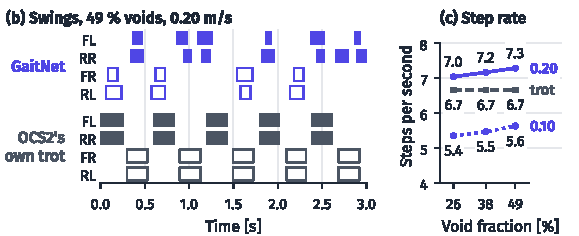
\includegraphics[width=0.7895\textwidth]{figures/fig_gait}% 120 of 152 mm
  \caption{Swings (bars) of GaitNet and OCS2's own trot in one successful
    trial each (world seed \corlGaitExampleSeed, \corlBenchVoidHigh\%
    voids, \corlBenchSpeedFast\,m/s), from when the rear feet reach the
    voids. Filled: front-left (FL) and rear-right (RR) legs; open:
    front-right (FR) and rear-left (RL).}
  \label{fig:gait}
\end{figure}

\looseness=-1 Fig.~\ref{fig:gait} shows the gait, from the
\corlGaitTrialsGaitNet{} successful trials of GaitNet and
\corlGaitTrialsTrot{} of the trot (App.~\ref{app:counts}). The trial of
Fig.~\ref{fig:gait}, at \corlBenchVoidHigh\% voids and
\corlBenchSpeedFast\,m/s, was not picked by hand: of the world seeds
that both methods passed in that cell, it is the one whose shares of
time with none, one, and two of GaitNet's feet up lie closest to the
cell's pooled shares. Swings come from the simulator's ground-truth foot
heights, logged about every 21\,ms of simulated time, so lift-off times
are known to about one tick. The statistics cover the time from when the
rear feet reach the voids to the end of each \corlBenchTrialSeconds\,s
trial; the front feet are already among the voids then. Failed trials
were not logged. Detected swings are shorter than commanded ones: the
trot's \corlTrotSwing\,s swings measure
\corlGaitTrotSwingMeasured\,s, while its \corlTrotPeriod\,s period
measures \corlGaitTrotPeriodMeasured\,s. For this reason the trot shows all four
feet down for \corlGaitAllDownTrot\% of the time, which its schedule
never has, and only comparisons between the two methods are meaningful.
GaitNet kept all four feet down for \corlGaitAllDownSlow\% of the time
at \corlBenchSpeedSlow\,m/s and \corlGaitAllDownFast\% at
\corlBenchSpeedFast\,m/s.
With two legs in swing, GaitNet's pair was diagonal for
\corlGaitDiagTimePct\% of the time, against 100\% for the trot. Of its
overlapping swing pairs, 227 paired the rear legs, 158 the legs of one
side, and 38 the front legs, against 24{,}370 diagonal pairs. Pairs of
other legs were most frequent in the hardest cell, \corlGaitNonDiagHard{}
per successful trial against \corlGaitNonDiagEasy{} at
\corlBenchVoidLow\% voids and \corlBenchSpeedSlow\,m/s, but they do not
mark where GaitNet-Diagonal loses success:
\corlGaitNonDiagMildTrials{} of the \corlGaitNonDiagMildOf{} successful
trials at \corlBenchVoidLow\% voids and \corlBenchSpeedFast\,m/s had at
least one, yet GaitNet-Diagonal lost nothing in that cell.

% ---------------------------------------------------------------------------
% Appendix: proofs for Sec. \ref{subsec:idm-theory}. Rewritten 2026-11-04
% (author: "remove the unnecessary stuff ... make the proofs more clear"):
% kept only what Sec. 4.4 uses; proofs in numbered steps. Removed (see git
% history, or scratchpad/appendix_idm_before_cleanup.tex of that session):
% the 2x2 counterexample to a Euclidean contraction, the noise-instantiation
% bound, the covariate-shift density bound, the Gaussian/sub-Gaussian tail
% bound (old Prop. (c)), the general one-sided covering, the union bound over
% a trial, and the tightness part (d) of the grid lemma with its numerical
% search. Numerical checks of the original: scratchpad/idmcheck/*.py.
% ---------------------------------------------------------------------------
\section{Analysis of the Inverse Footstep Model}
\label{app:idm-proofs}

\looseness=-1 This appendix proves the statements of
Sec.~\ref{subsec:idm-theory}: when the regression of
Eq.~\eqref{eq:idm-loss} inverts the controller (Proposition~\ref{prop:idm-mean}),
how it is biased otherwise (Proposition~\ref{prop:idm-shrink}), when a
landing error can put the foot in a void (Proposition~\ref{prop:idm-void}),
and how much clearance the grown mask leaves (Lemma~\ref{lem:idm-grid}).
We drop the superscript $c$ from $I^c$. Let $P_c$ be the distribution of the
logged tuples $(\zeta, \mathbf u, \mathbf o)$, one per step the controller
executed, and $I_\star(\zeta,\mathbf o) := \mathbb E_{P_c}[\mathbf u \mid
\zeta,\mathbf o]$ the function the regression estimates. Norms are
Euclidean unless marked, $\mathrm{Id}$ is the identity matrix, and $\Phi$
is the standard normal distribution function. We assume $\mathbb
E_{P_c}\|\mathbf u\|^2 < \infty$ throughout.

\looseness=-1 Throughout, we assume that the law of the landing $\mathbf o$
given $(\zeta,\mathbf u)$ is the same when logging and at deployment,
although the logging policy and GaitNet both choose commands from terrain
that $\zeta$ omits. Two parts of our pipeline strain our assumptions. The
training controller's IDM is fitted without the controller randomization
it later runs under (Sec.~\ref{subsec:method-training}), which changes
that law. The OCS2 IDM is fitted on steps sent through the training
controller's IDM, so its logged landings need not cover the deployed
targets, as Assumption~\ref{as:idm-exact}(iii) below requires; logging
again with the deployed IDM \citep{christiano_transfer_2016} would reduce
this gap.

\subsection{When the Regression Inverts the Controller}

\begin{assumption}[Exact relabelling]
\label{as:idm-exact}
(i)~There is no residual: the landing is $\mathbf o = \bar
F_c(\zeta,\mathbf u)$ for every $(\zeta,\mathbf u)$ in the support of the
logged pairs, when logging and at deployment.
(ii)~For every $(\zeta,\mathbf o)$, the commands $\mathbf u$ with
$(\zeta,\mathbf u)$ in that support and $\bar F_c(\zeta,\mathbf u) =
\mathbf o$ form a convex set.
(iii)~Every deployment pair $(\zeta,\mathbf u^\star)$ lies in the support
of the logged $(\zeta,\mathbf o)$, and $\bar F_c$ (on the support of the
logged pairs) and $I_\star$ have continuous versions, which we use.
(iv)~The fitted IDM $I$ is continuous and equals $I_\star$ $P_c$-almost
everywhere.
\end{assumption}

Condition (ii) holds, with single points, whenever the landing offset
changes less than the command, that is, when $\mathbf u \mapsto \bar
F_c(\zeta,\mathbf u) - \mathbf u$ is Lipschitz with a constant below one
(step~5 of the proof below).

\begin{proposition}[Hindsight regression]
\label{prop:idm-mean}
(a)~Among the square-integrable functions of $(\zeta,\mathbf o)$,
$I_\star$ minimises the loss of Eq.~\eqref{eq:idm-loss}, uniquely up to
$P_c$-null sets.
(b)~Under Assumption~\ref{as:idm-exact}, every deployment pair has
$\bar F_c(\zeta, I(\zeta,\mathbf u^\star))$ $= \mathbf u^\star$, so the foot
lands at $\mathbf u^\star$.
\end{proposition}

Every logged step is an example of the inverse map, since its command
landed the foot at $\mathbf o$; noise added to a command before it is
sent therefore does not corrupt its label. Each condition of
Assumption~\ref{as:idm-exact} matters. Without (i), the regression averages
$\mathbf u$ over the hidden states that share $(\zeta,\mathbf o)$ and is
biased even with unlimited data \citep{eysenbach_imitating_2022}
(Proposition~\ref{prop:idm-shrink}). Without (ii), commands from two
inverse branches that land at the same point can average to one that
lands at neither \citep{jordan_forward_1992}. Without (iii), the held-out
error says nothing about targets outside the logged landings.

\begin{idmproof}{Proposition~\ref{prop:idm-mean}}
(a)~For a square-integrable $I$, split $\mathbf u - I = (\mathbf u -
I_\star) + (I_\star - I)$. The cross term vanishes, $\mathbb E[(\mathbf u -
I_\star)^\top(I_\star - I)] = \mathbb E\big[\mathbb E[\mathbf u - I_\star
\mid \zeta,\mathbf o]^\top (I_\star - I)\big] = 0$, because $I_\star - I$
depends only on $(\zeta,\mathbf o)$ and $\mathbb E[\mathbf u - I_\star
\mid \zeta,\mathbf o] = \mathbf 0$. Hence
\begin{equation}
  \mathbb E\|\mathbf u - I\|^2 = \mathbb E\|\mathbf u - I_\star\|^2
  + \mathbb E\|I_\star - I\|^2 ,
  \label{eq:app-orth}
\end{equation}
which is smallest exactly when $I = I_\star$ almost everywhere. In words,
the held-out squared error of any IDM is the irreducible error plus its
mean squared distance from $I_\star$.

(b)~We use that the support of a distribution is the smallest closed
set of probability one, so a closed set of probability one contains it.

\emph{Step 1: the logged commands for a landing.} Let $\mathcal
U(\zeta,\mathbf o)$ be the set of commands $\mathbf u$ with $(\zeta,\mathbf
u)$ in the support of the logged pairs and $\bar F_c(\zeta,\mathbf u) =
\mathbf o$. It is closed because the support is closed and $\bar F_c$ is
continuous, and convex by (ii). Logged pairs lie in their support and, by
(i), land at $\bar F_c(\zeta,\mathbf u)$, so given $(\zeta,\mathbf o)$ the
command lies in $\mathcal U(\zeta,\mathbf o)$ with probability one.

\emph{Step 2: the mean stays in the set.} The mean of a distribution that
gives probability one to a closed convex set lies in that set: if the
mean $\bar{\mathbf x}$ were outside, a separating hyperplane would give a vector
$\boldsymbol\nu$ and a number $t$ with $\boldsymbol\nu^\top\bar{\mathbf x} > t
\ge \boldsymbol\nu^\top\mathbf x$ for every $\mathbf x$ in the set, and
taking the mean of the second inequality would give
$\boldsymbol\nu^\top\bar{\mathbf x} \le t$. Applied to the conditional
distribution of $\mathbf u$ given $(\zeta,\mathbf o)$, this gives
$I_\star(\zeta,\mathbf o) \in \mathcal U(\zeta,\mathbf o)$, so $\bar
F_c(\zeta, I_\star(\zeta,\mathbf o)) = \mathbf o$ for $P_c$-almost every
$(\zeta,\mathbf o)$.

\emph{Step 3: from almost every landing to every target.} By step~2,
the set of $(\zeta,\mathbf o)$ with $(\zeta, I_\star(\zeta,\mathbf o))$ in
the support of the logged pairs and $\bar F_c(\zeta, I_\star(\zeta,\mathbf
o)) = \mathbf o$ has probability one. It is closed, as $I_\star$ and $\bar
F_c$ are continuous by (iii), so it contains the support of the logged
$(\zeta,\mathbf o)$, and with it every deployment pair $(\zeta,\mathbf
u^\star)$. Hence the command $I_\star(\zeta,\mathbf u^\star)$ lies in the
support of the logged pairs and $\bar F_c(\zeta, I_\star(\zeta,\mathbf
u^\star)) = \mathbf u^\star$.

\emph{Step 4: the fitted IDM.} By (iv), the set where the continuous $I$
equals $I_\star$ is closed and has probability one, so it contains the
support, and $I(\zeta,\mathbf u^\star) = I_\star(\zeta,\mathbf u^\star)$.
This command lies in the support of the logged pairs, where by (i) the
landing equals $\bar F_c$, so the foot lands at $\mathbf u^\star$.

\emph{Step 5: the condition after the assumption.} If $\mathbf u \mapsto
\bar F_c(\zeta,\mathbf u) - \mathbf u$ is $L_\delta$-Lipschitz with
$L_\delta < 1$, then $\|\bar F_c(\zeta,\mathbf u) - \bar F_c(\zeta,\mathbf
u')\| \ge \|\mathbf u - \mathbf u'\| - L_\delta\|\mathbf u - \mathbf u'\| >
0$ for $\mathbf u \ne \mathbf u'$, so $\bar F_c(\zeta,\cdot)$ is injective
and every $\mathcal U(\zeta,\mathbf o)$ has at most one point.
\end{idmproof}

\subsection{Bias When the Landings Are Noisy}

\begin{proposition}[Relabelling bias]
\label{prop:idm-shrink}
Fix $\zeta$. Let the logged commands be $\mathbf u \sim \mathcal
N(\boldsymbol\mu,\Sigma_u)$ with $\Sigma_u \succ 0$, and the landings
$\mathbf o = A\mathbf u + \mathbf b + \boldsymbol\eta$ with $A$ invertible
and $\boldsymbol\eta \sim \mathcal N(\mathbf 0,\Sigma_\eta)$ independent
of $\mathbf u$. Let $\bar{\mathbf o} = A\boldsymbol\mu + \mathbf b$ be the
mean logged landing and $S = A\Sigma_u A^\top + \Sigma_\eta$ the covariance
of the logged landings. For a target $\mathbf u^\star$, the landing
$\mathbf o^\star$ of the command $I_\star(\zeta,\mathbf u^\star)$ has the
mean error
\begin{equation}
  \mathbb E[\mathbf o^\star] - \mathbf u^\star
  = -\Lambda\,(\mathbf u^\star - \bar{\mathbf o}), \qquad
  \Lambda = \Sigma_\eta S^{-1}.
  \label{eq:idm-shrink}
\end{equation}
The eigenvalues of $\Lambda$ lie in $[0,1)$, and
$\|\mathbb E[\mathbf o^\star] - \bar{\mathbf o}\|_{S^{-1}} \le \|\mathbf
u^\star - \bar{\mathbf o}\|_{S^{-1}}$, with $\|\mathbf x\|_{S^{-1}}^2 :=
\mathbf x^\top S^{-1}\mathbf x$. A larger $\Sigma_u$ (in the
positive-semidefinite order) raises no eigenvalue of $\Lambda$.
\end{proposition}

\looseness=-1 Here $\Sigma_\eta$ is the part of the landing covariance $S$
that the command does not explain. In one dimension, $\Lambda$ is that
share of the landing variance, and the deployed landing falls short of
$\mathbf u^\star$, toward the mean logged landing $\bar{\mathbf o}$, by
the fraction $\Lambda$ of their distance. In the plane, the pull toward
$\bar{\mathbf o}$ holds in the metric $\|\cdot\|_{S^{-1}}$ of the logged
landings, not necessarily in the Euclidean one, and the bias, measured
in that metric, is at most the largest eigenvalue of $\Lambda$ times
$\|\mathbf u^\star - \bar{\mathbf o}\|_{S^{-1}}$, so it can be largest for footholds that the logging policy
seldom reached. This is the attenuation bias of a regression on a noisy
input. Spreading the logged commands raises no eigenvalue of $\Lambda$,
and in one dimension it shrinks the bias, a second reason, besides
coverage, for the command noise in the training controller's IDM data
(App.~\ref{app:settings});
in the plane, the bias at a given target can still grow.

\begin{idmproof}{Proposition~\ref{prop:idm-shrink}}
\emph{Step 1: the regression is linear.} $(\mathbf u,\mathbf o)$ is
jointly Gaussian with $\operatorname{Cov}(\mathbf o) = S \succ 0$ and
$\operatorname{Cov}(\mathbf u,\mathbf o) = \Sigma_u A^\top$, so
$I_\star(\zeta,\mathbf o) = \boldsymbol\mu + W(\mathbf o - \bar{\mathbf
o})$ with the gain $W = \Sigma_u A^\top S^{-1}$.

\emph{Step 2: the mean landing.} The command $\tilde{\mathbf u} =
I_\star(\zeta,\mathbf u^\star)$ is fixed at the decision and
$\boldsymbol\eta$ is independent of it, so $\mathbb E[\mathbf o^\star] =
A\tilde{\mathbf u} + \mathbf b = \bar{\mathbf o} + AW(\mathbf u^\star -
\bar{\mathbf o})$. Hence $\mathbb E[\mathbf o^\star] - \mathbf u^\star =
-(\mathrm{Id} - AW)(\mathbf u^\star - \bar{\mathbf o})$, and $\mathrm{Id} -
AW = (S - A\Sigma_u A^\top)S^{-1} = \Sigma_\eta S^{-1} = \Lambda$.

\emph{Step 3: the eigenvalues.} Let $M := S^{-1/2}\Sigma_\eta S^{-1/2} =
\mathrm{Id} - S^{-1/2}A\Sigma_u A^\top S^{-1/2}$. It is symmetric, positive
semidefinite because $\Sigma_\eta \succeq 0$, and $M \prec \mathrm{Id}$ because
$A\Sigma_u A^\top \succ 0$, so its eigenvalues lie in $[0,1)$. Since
$\Lambda = S^{1/2} M S^{-1/2}$, $\Lambda$ has the same eigenvalues.

\emph{Step 4: the contraction.} $\mathbb E[\mathbf o^\star] - \bar{\mathbf
o} = (\mathrm{Id} - \Lambda)(\mathbf u^\star - \bar{\mathbf o})$ and
$S^{-1/2}(\mathrm{Id} - \Lambda) = (\mathrm{Id} - M)S^{-1/2}$. As $0 \prec
\mathrm{Id} - M \preceq \mathrm{Id}$, $\|\mathbb E[\mathbf o^\star] -
\bar{\mathbf o}\|_{S^{-1}} = \|(\mathrm{Id} - M)S^{-1/2}(\mathbf u^\star -
\bar{\mathbf o})\| \le \|S^{-1/2}(\mathbf
u^\star - \bar{\mathbf o})\| = \|\mathbf u^\star - \bar{\mathbf
o}\|_{S^{-1}}$. In the same way, $\|S^{-1/2}\Lambda(\mathbf u^\star -
\bar{\mathbf o})\| = \|M S^{-1/2}(\mathbf u^\star - \bar{\mathbf o})\| \le
\lambda_{\max}(M)\,\|\mathbf u^\star - \bar{\mathbf o}\|_{S^{-1}}$, which
bounds the bias in the metric $\|\cdot\|_{S^{-1}}$.

\emph{Step 5: more command spread.} The eigenvalues of $\Lambda =
\Sigma_\eta S^{-1}$ equal those of the symmetric matrix
$\Sigma_\eta^{1/2}S^{-1}\Sigma_\eta^{1/2}$, since $XY$ and $YX$ have the
same eigenvalues. A larger $\Sigma_u$ gives a larger $S$ and so a smaller
$S^{-1}$ and a smaller $\Sigma_\eta^{1/2}S^{-1}\Sigma_\eta^{1/2}$, whose
ordered eigenvalues therefore do not increase.
\end{idmproof}

\subsection{Landing Error and Voids}

\begin{proposition}[Landing error and voids]
\label{prop:idm-void}
For the command $\mathbf u = I(\zeta,\mathbf u^\star)$ and the clearance
$d(\mathbf u^\star)$ of Sec.~\ref{subsec:idm-theory}, let $\mathcal G$ be
the information at the decision, which fixes $\zeta$, $\mathbf u^\star$,
$\mathbf u$ and $\mathcal V$, and let $\boldsymbol\beta := \bar
F_c(\zeta,\mathbf u) - \mathbf u^\star$. Then the landing error is
$\mathbf e := \mathbf o - \mathbf u^\star = \boldsymbol\beta +
\boldsymbol\eta$, and
(a)~if $\|\boldsymbol\beta\| + \|\boldsymbol\eta\| < d(\mathbf u^\star)$,
the foot does not land in a void;
(b)~$\Pr(\mathbf o \in \mathcal V \mid \mathcal G) \le \Pr(\|\mathbf
e\|_\infty \ge d(\mathbf u^\star) \mid \mathcal G)$.
\end{proposition}

\begin{idmproof}{Proposition~\ref{prop:idm-void}}
By Eq.~\eqref{eq:mean-forward}, $\mathbf e = \bar F_c(\zeta,\mathbf u) +
\boldsymbol\eta - \mathbf u^\star = \boldsymbol\beta + \boldsymbol\eta$. As $\boldsymbol\eta$ has mean zero given
$(\zeta,\mathbf u)$, the mean error is $\boldsymbol\beta$, so an IDM with
the inputs $\zeta$ can cancel at most $\boldsymbol\beta$.
If $\mathbf o \in \mathcal V$, then, since $d(\mathbf u^\star)$ is the
$\infty$-norm distance from $\mathbf u^\star$ to the nearest void point,
$d(\mathbf u^\star) \le \|\mathbf o - \mathbf u^\star\|_\infty = \|\mathbf
e\|_\infty \le \|\mathbf e\| \le \|\boldsymbol\beta\| +
\|\boldsymbol\eta\|$. Read backwards, this is (a). It also shows $\{\mathbf
o \in \mathcal V\} \subseteq \{\|\mathbf e\|_\infty \ge d(\mathbf
u^\star)\}$, which is (b). Both statements weaken as $d$ shrinks, so a
lower bound on $d(\mathbf u^\star)$, such as that of
Lemma~\ref{lem:idm-grid}, may replace it.
\end{idmproof}

\paragraph{Where $\boldsymbol\beta$ comes from.}
\looseness=-1 With $\tilde{\mathbf u} := I_\star(\zeta,\mathbf u^\star)$,
\begin{equation}
  \boldsymbol\beta = \big[\bar F_c(\zeta,\mathbf u) - \bar
  F_c(\zeta,\tilde{\mathbf u})\big] + \big[\bar F_c(\zeta,\tilde{\mathbf
  u}) - \mathbf u^\star\big].
  \label{eq:app-beta}
\end{equation}
If $\bar F_c(\zeta,\cdot)$ is $L$-Lipschitz on the segment from
$\tilde{\mathbf u}$ to $\mathbf u$, the first term is at most
$L\|I(\zeta,\mathbf u^\star) - I_\star(\zeta,\mathbf u^\star)\|$: the
IDM's fitting error, whose mean square over the logged landings is its
held-out error minus the irreducible error (Eq.~\eqref{eq:app-orth}); at
a given target, the held-out error speaks for it only where the logged
landings cover that target (Assumption~\ref{as:idm-exact}(iii)). In the form of
Eq.~\eqref{eq:forward}, $\bar F_c(\zeta,\mathbf u) = \mathbf u +
\mathbb E[\boldsymbol\delta_c \mid \zeta,\mathbf u]$, so a landing offset
that depends only weakly on the command gives $L \approx 1$. The second
term, the relabelling bias, vanishes under Assumption~\ref{as:idm-exact}
(steps 1--3 of the proof of Proposition~\ref{prop:idm-mean}) and equals
$-\Lambda(\mathbf u^\star - \bar{\mathbf o})$ in the setting of
Proposition~\ref{prop:idm-shrink}.

\begin{remark}[Landing error against the margin]
\label{rem:idm-numbers}
On flat ground, the IDM cut OCS2's landing error from
\corlOcsLandRmsNoIdm\ to \corlOcsLandRmsIdm\,cm RMS
(Sec.~\ref{subsec:exp-why}). Suppose $\mathbf e$ is zero-mean isotropic
Gaussian with standard deviation $\sigma$ per axis. A foothold whose
nearest void lies beyond a long straight edge at Euclidean distance
$c_\perp$ then lands in it with probability $\Phi(-c_\perp/\sigma)$,
because only the error component normal to the edge matters. An edge at
$\infty$-norm distance $d$ with unit normal $\mathbf n$ has $c_\perp =
d\|\mathbf n\|_1 \ge d$. For our candidates, Lemma~\ref{lem:idm-grid}(c)
with $k = 2$ gives, with $\varphi$ the angle between the void edges
and the grid axes, for $0 \le \varphi \le 45^\circ$ and by symmetry at every angle, $c_\perp \ge (2 - \tfrac12\sin 2\varphi)(\sin\varphi +
\cos\varphi)\,h \ge 2h = m$, with equality for edges parallel to the grid,
so such an edge at $d = m$ is the worst straight edge. The
\corlOcsLandRmsIdm\,cm is the RMS of $\|\mathbf e\|$, so $\sigma =
\sqrt2$\,cm, and at $d = \corlMarginCm$\,cm, the margin, this probability
is $\Phi(-\sqrt2) \approx 0.079$. If ten of the roughly 97 footholds of a
sweep trial (\corlOcsStepsPerMFull{} steps per metre over
\corlOcsTrackM\,m) were this close to an edge, with independent errors,
the trial would stay void-free with probability only $(1 - 0.079)^{10}
\approx 0.44$. At a pillar corner, with voids beyond two perpendicular
edges at distance $d$, a foothold lands in a void with probability $1 - (1
- 0.079)^2 \approx 0.15$. We have
not measured how close GaitNet's footholds come to voids.
\end{remark}

\subsection{Clearance of the Grown Mask}

\looseness=-1 Model the terrain rays as samples on the lattice $\mathbf
r_0 + h\mathbb Z^2$ in the yaw frame of the decision, a sample being unsafe
if it lies in the closed void set $\mathcal V$ (exact perception and
registration). A candidate is a sample with no unsafe sample within
$\infty$-norm distance $kh$; this is the grown mask, a $(2k{+}1)\times
(2k{+}1)$ max-pool without padding, so every lattice point within $kh$ of a
candidate is sampled. Let
\[
  \rho_{\mathcal V} := \sup_{\mathbf p \in \mathcal V}\;
  \min\big\{\|\mathbf p - \mathbf r\|_\infty :
  \mathbf r \in (\mathbf r_0 + h\mathbb Z^2) \cap \mathcal V\big\}
\]
be the largest distance from a void point to the nearest lattice point in
the void (with $\rho_{\mathcal V} = \infty$, and Lemma~\ref{lem:idm-grid}(a)
empty, if part of the void holds no lattice point).

\begin{lemma}[Clearance]
\label{lem:idm-grid}
(a)~Every candidate $\mathbf u^\star$ has $d(\mathbf u^\star) \ge (k+1)h -
\rho_{\mathcal V}$.
(b)~If $\mathcal V$ is a union of closed rectangles with sides parallel to
the grid axes and at least $h$ long, then $\rho_{\mathcal V} \le h$, so
$d(\mathbf u^\star) \ge kh = m$.
(c)~If $\mathcal V$ is a union of closed squares of side at least
$2\sqrt2\,h$ whose edges make an angle $\varphi$ with the grid axes, then
$\rho_{\mathcal V} \le (1 + \tfrac12|\sin 2\varphi|)\,h$, so $d(\mathbf
u^\star) \ge (k - \tfrac12|\sin 2\varphi|)\,h$. For squares at different
angles, take the largest $|\sin 2\varphi|$.
\end{lemma}

\begin{idmproof}{Lemma~\ref{lem:idm-grid}}
(a)~Take a void point $\mathbf p$ and a lattice point $\mathbf r$ in the
void with $\|\mathbf p - \mathbf r\|_\infty \le \rho_{\mathcal V}$ (a
nearest one exists, as only finitely many lattice points lie within any
distance). If $\|\mathbf r - \mathbf u^\star\|_\infty \le kh$, then
$\mathbf r$ would be sampled, hence unsafe, within $kh$ of the candidate
$\mathbf u^\star$, which the mask excludes. So $\|\mathbf r - \mathbf
u^\star\|_\infty > kh$, and since both are lattice points, $\|\mathbf r -
\mathbf u^\star\|_\infty \ge (k+1)h$. By the triangle inequality, $\|\mathbf
p - \mathbf u^\star\|_\infty \ge (k+1)h - \rho_{\mathcal V}$ for every void
point $\mathbf p$.

(b)~Work on one axis. Let $\mathbf p$ lie in a rectangle whose side along
that axis is $[a,b]$, $b - a \ge h$, and let $t^- \le p \le t^+$ be the
lattice coordinates next to $p$, so $t^+ - t^- \le h$. If $t^- \ge a$, then
$t^- \in [a,b]$. Otherwise $t^+ \le t^- + h < a + h \le b$ and $t^+ \ge p \ge
a$, so $t^+ \in [a,b]$. Either way, a lattice coordinate in $[a,b]$ lies
within $h$ of $p$. Doing this on both axes gives a lattice point in the
rectangle within $\infty$-norm distance $h$ of $\mathbf p$.

(c)~\emph{Step 1: reduction.} Take $\mathbf p$ in a square $\mathcal Q
\subseteq \mathcal V$ of side $s \ge 2\sqrt2\,h$. Reflections in the grid
axes and the diagonal map the lattice to a translate of itself and
preserve $\|\cdot\|_\infty$, so we may take $h = 1$ and $0 \le \varphi \le
45^\circ$, and, moving the lattice, $\mathbf p = \mathbf 0$. Let $\mathbf d_1
= (\cos\varphi, \sin\varphi)$ and $\mathbf d_2 = (-\sin\varphi,
\cos\varphi)$ be the edge directions. $\mathcal Q$ extends at least $s/2$
from $\mathbf p$ along one of $\pm\mathbf d_1$ and one of $\pm\mathbf d_2$.
Rotations by multiples of $90^\circ$ about $\mathbf p$ permute these four
signed directions cyclically, keep $\varphi$, and also map the lattice to
a translate of itself, so we may take the two directions to be $+\mathbf
d_1$ and $+\mathbf d_2$. Then $\mathcal Q$ contains the quarter square
$\mathcal W := \{\gamma_1 \mathbf d_1 + \gamma_2\mathbf d_2 : 0 \le
\gamma_1,\gamma_2 \le s/2\}$.

\emph{Step 2: an axis-aligned unit square inside $\mathcal W$.} Let $B :=
[x_0, x_0+1] \times [y_0, y_0+1]$ with $x_0 = -\sin^2\varphi$ and $y_0 =
\sin\varphi\cos\varphi$. Its lower corners are $(\cos^2\varphi, y_0) =
\cos\varphi\,\mathbf d_1$ and $(x_0, y_0) = \sin\varphi\,\mathbf d_2$, and
its upper corners add $(0,1) = \sin\varphi\,\mathbf d_1 +
\cos\varphi\,\mathbf d_2$. In the coordinates $(\gamma_1,\gamma_2)$, the
four corners are $(\cos\varphi, 0)$, $(0, \sin\varphi)$, $(\cos\varphi +
\sin\varphi, \cos\varphi)$ and $(\sin\varphi, \sin\varphi + \cos\varphi)$:
all have $0 \le \gamma_1, \gamma_2 \le \sin\varphi + \cos\varphi \le \sqrt2
\le s/2$. By convexity, $B \subseteq \mathcal W \subseteq \mathcal Q$, and
every point of $B$ lies within $\infty$-norm distance $\max(\sin^2\varphi,
\cos^2\varphi, 1 + y_0) = 1 + \tfrac12\sin 2\varphi$ of $\mathbf 0$.

\emph{Step 3: a lattice point in $B$.} A closed axis-aligned unit square
contains a point of every translate of $\mathbb Z^2$, because a closed unit
interval contains a point of every translate of $\mathbb Z$. So $\mathcal Q$
contains a lattice point within $\infty$-norm distance $1 + \tfrac12\sin
2\varphi$ of $\mathbf p$. As $\mathbf p$ was any void point, this bounds
$\rho_{\mathcal V}$, and part (a) gives the clearance.
\end{idmproof}

\looseness=-1 Our tiles, $12.5h$ wide in Isaac and Gazebo, meet the side
condition $2\sqrt2\,h \approx 2.8h$. With $k = 2$ and $h = 1$\,cm, every
candidate therefore has a clearance of at least $(2 - \tfrac12|\sin
2\varphi|)$\,cm, that is, $2$\,cm for edges parallel to the grid and
$1.5$\,cm at $45^\circ$. The lemma assumes exact terrain. It ignores the
foot's size, and at deployment, where the grid is resampled from a
depth-camera map that keeps its own distance from unwalkable cells
(App.~\ref{app:deployment}), it does not cover that map's errors.

